\documentclass[landscape,a0paper,fontscale=0.285]{baposter}

\usepackage{relsize}
\usepackage{url}
\usepackage{graphicx}
\usepackage{multicol}
\usepackage{amsmath}
\usepackage{amssymb}
\usepackage{enumitem}
\usepackage{xcolor}
\usepackage{tikz}
\usetikzlibrary{shapes,arrows,positioning,calc}

% Color definitions - Academic theme
\definecolor{navyblue}{RGB}{26,54,93}
\definecolor{forestgreen}{RGB}{39,103,73}
\definecolor{brickred}{RGB}{197,48,48}
\definecolor{goldaccent}{RGB}{214,158,46}
\definecolor{lightgray}{RGB}{247,250,252}
\definecolor{lightblue}{RGB}{235,241,250}
\definecolor{lightgreen}{RGB}{235,250,241}
\definecolor{lightred}{RGB}{253,240,240}
\definecolor{lightyellow}{RGB}{255,250,235}
\definecolor{darktext}{RGB}{45,55,72}

\begin{document}

\begin{poster}{
    % Poster Options
    grid=false,
    columns=4,
    colspacing=0.8em,
    bgColorOne=white,
    bgColorTwo=white,
    borderColor=navyblue,
    headerColorOne=navyblue,
    headerColorTwo=navyblue,
    headerFontColor=white,
    boxColorOne=white,
    boxColorTwo=lightgray,
    textborder=rounded,
    eyecatcher=true,
    headerborder=closed,
    headerheight=0.08\textheight,
    headershape=rounded,
    headershade=plain,
    headerfont=\Large\bf\textsf,
    boxshade=plain,
    background=plain,
    linewidth=2pt
}
% Eye Catcher (Left logo)
{
    
\begin{tikzpicture}[scale=1.2]
        \draw[navyblue, ultra thick] (0,0) sin (0.4,0.4) cos (0.8,0) sin (1.2,-0.4) cos (1.6,0) sin (2,0.4) cos (2.4,0);
        \draw[forestgreen, ultra thick, line width=3pt] (0,0) -- (0.4,0.08) -- (0.8,0.04) -- (1.2,-0.08) -- (1.6,0) -- (2,0.12) -- (2.4,0.04);
    \end{tikzpicture}
}
% Title
{
    \textsf{\textbf{\Huge Kalman Filter: A Probabilistic Approach to Signal Estimation and Noise Reduction}}
}
% Authors
{
    \textsf{\Large Probability \& Statistics Course --- Final Project}\\[0.3em]
    \textsf{\large Demo: \url{https://leonathn.github.io/FinalProjectProbability/}}
}
% University Logo (Right)
{
    
\begin{tikzpicture}[scale=0.8]
        \node[circle, draw=navyblue, line width=3pt, minimum size=2.5cm, font=\Large\bfseries] {P\&S};
    \end{tikzpicture}
}

%==============================================================================
% COLUMN 1: INTRODUCTION & THEORY
%==============================================================================

\headerbox{\textsf{1. Introduction \& Problem}}{name=intro,column=0,row=0}{
\small
In real-world applications, measurements are always corrupted by \textbf{noise}. The Kalman Filter provides an \textbf{optimal solution} to estimate the true value.

\vspace{0.5em}
\colorbox{lightblue}{\parbox{0.95\linewidth}{
\textbf{Problem Statement:}
\begin{equation*}
z_k = x_k + v_k
\end{equation*}
\begin{itemize}[leftmargin=*, nosep, topsep=2pt]
    \item $z_k$ = noisy measurement
    \item $x_k$ = true (unknown) value
    \item $v_k \sim \mathcal{N}(0, R)$ = noise
\end{itemize}
}}

\vspace{0.5em}
\textbf{Goal:} Find $\hat{x}_k$ that minimizes estimation error variance.

\vspace{0.5em}
\textit{Developed by Rudolf E. Kálmán in 1960}
}

\headerbox{\textsf{2. Probability Foundations}}{name=probability,column=0,below=intro}{
\small
\colorbox{lightgreen}{\parbox{0.95\linewidth}{
\textbf{\textcolor{forestgreen}{Gaussian Distribution:}}
\begin{equation*}
p(x) = \frac{1}{\sqrt{2\pi\sigma^2}} \exp\left(-\frac{(x-\mu)^2}{2\sigma^2}\right)
\end{equation*}
}}

\vspace{0.4em}
\colorbox{lightyellow}{\parbox{0.95\linewidth}{
\textbf{\textcolor{goldaccent}{Variance = Uncertainty:}}
\begin{equation*}
\text{Var}(X) = \sigma^2 = E[(X - \mu)^2]
\end{equation*}
}}

\vspace{0.4em}
\colorbox{lightred}{\parbox{0.95\linewidth}{
\textbf{\textcolor{brickred}{Bayes' Theorem:}}
\begin{equation*}
P(A|B) = \frac{P(B|A) \cdot P(A)}{P(B)}
\end{equation*}
}}

\vspace{0.3em}
The Kalman Filter is \textbf{recursive Bayesian estimation}!
}

\headerbox{\textsf{Keywords}}{name=keywords,column=0,below=probability}{
\footnotesize
\textbf{Kalman Filter} $\bullet$ \textbf{Bayesian Estimation} $\bullet$ \textbf{Gaussian} $\bullet$ \textbf{Variance} $\bullet$ \textbf{Signal Processing} $\bullet$ \textbf{Noise Reduction}
}

%==============================================================================
% COLUMN 2: THE ALGORITHM
%==============================================================================

\headerbox{\textsf{3. The Kalman Filter Algorithm}}{name=algorithm,column=1,row=0,span=1}{
\small
The filter operates in two phases: \textbf{Predict} $\rightarrow$ \textbf{Update}

\vspace{0.3em}
\begin{center}
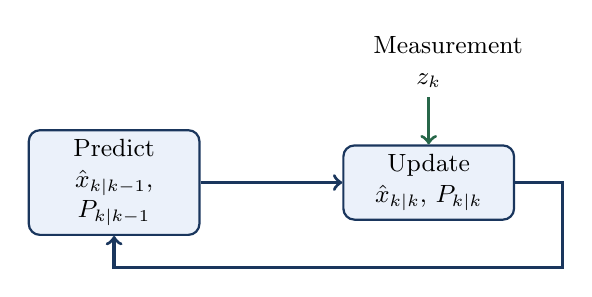
\begin{tikzpicture}[node distance=1.8cm, auto,
    block/.style={rectangle, draw=navyblue, thick, fill=lightblue, text width=5.5em, text centered, rounded corners, minimum height=2.5em, font=\small},
    arrow/.style={->, very thick, navyblue}]
    
    \node[block] (predict) {Predict\\$\hat{x}_{k|k-1}$, $P_{k|k-1}$};
    \node[block, right=of predict] (update) {Update\\$\hat{x}_{k|k}$, $P_{k|k}$};
    \node[above=0.6cm of update, text width=4em, text centered, font=\small] (meas) {Measurement\\$z_k$};
    
    \draw[arrow] (predict) -- (update);
    \draw[arrow] (update.east) -- ++(0.6,0) |- ([yshift=-0.4cm]predict.south) -- (predict.south);
    \draw[arrow, forestgreen] (meas) -- (update);
\end{tikzpicture}
\end{center}

\vspace{0.3em}
\colorbox{lightblue}{\parbox{0.95\linewidth}{
\textbf{\textcolor{navyblue}{Step 1: Prediction}}
\begin{align*}
\hat{x}_{k|k-1} &= \hat{x}_{k-1|k-1}\\
P_{k|k-1} &= P_{k-1|k-1} + Q
\end{align*}
}}

\vspace{0.3em}
\colorbox{lightgreen}{\parbox{0.95\linewidth}{
\textbf{\textcolor{forestgreen}{Step 2: Kalman Gain}}
\begin{equation*}
\boxed{K_k = \frac{P_{k|k-1}}{P_{k|k-1} + R}}
\end{equation*}
\centering\small $K$ = how much to trust measurement
}}

\vspace{0.3em}
\colorbox{lightyellow}{\parbox{0.95\linewidth}{
\textbf{\textcolor{goldaccent}{Step 3: State Update}}
\begin{equation*}
\boxed{\hat{x}_{k|k} = \hat{x}_{k|k-1} + K_k(z_k - \hat{x}_{k|k-1})}
\end{equation*}
\centering\small Weighted average!
}}

\vspace{0.3em}
\colorbox{lightred}{\parbox{0.95\linewidth}{
\textbf{\textcolor{brickred}{Step 4: Covariance Update}}
\begin{equation*}
\boxed{P_{k|k} = (1 - K_k) P_{k|k-1}}
\end{equation*}
\centering\small Uncertainty decreases!
}}
}

\headerbox{\textsf{4. Intuitive Understanding}}{name=intuition,column=1,below=algorithm}{
\small
\textbf{The Kalman Gain as ``Trust Factor'':}

\vspace{0.3em}
\begin{center}
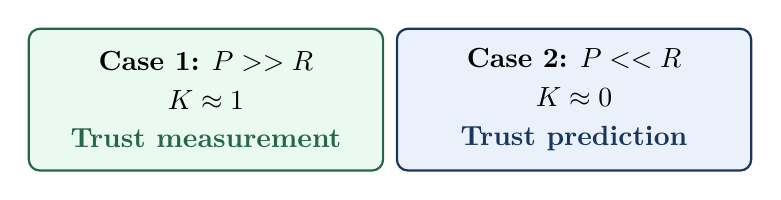
\begin{tikzpicture}[scale=0.85]
    \node[draw=forestgreen, thick, fill=lightgreen, rounded corners, minimum width=4.5cm, minimum height=1.8cm, align=center] at (0,0) {
        \textbf{Case 1:} $P >> R$\\[2pt]
        $K \approx 1$\\[2pt]
        \textcolor{forestgreen}{\textbf{Trust measurement}}
    };
    \node[draw=navyblue, thick, fill=lightblue, rounded corners, minimum width=4.5cm, minimum height=1.8cm, align=center] at (5.5,0) {
        \textbf{Case 2:} $P << R$\\[2pt]
        $K \approx 0$\\[2pt]
        \textcolor{navyblue}{\textbf{Trust prediction}}
    };
\end{tikzpicture}
\end{center}

\vspace{0.3em}
\textbf{GPS Analogy:} This is why GPS dots move \textbf{smoothly}!
}

%==============================================================================
% COLUMN 3: EXAMPLE & VISUALIZATION
%==============================================================================

\headerbox{\textsf{5. Numerical Example}}{name=example,column=2,row=0}{
\small
\colorbox{lightgray}{\parbox{0.95\linewidth}{
\textbf{Given:} $\hat{x}_{k-1} = 100$, $P_{k-1} = 4$, $z_k = 105$, $Q = 1$, $R = 10$
}}

\vspace{0.4em}
\begin{center}
\begin{tabular}{|l|l|c|}
\hline
\textbf{Step} & \textbf{Calculation} & \textbf{Result} \\
\hline
\cellcolor{lightblue}Predict $P$ & $4 + 1$ & $P = 5$ \\
\hline
\cellcolor{lightgreen}Kalman Gain & $\frac{5}{5+10}$ & $K = \textcolor{forestgreen}{\mathbf{0.333}}$ \\
\hline
\cellcolor{lightyellow}Update $\hat{x}$ & $100 + 0.333(105-100)$ & $\hat{x} = \textcolor{goldaccent}{\mathbf{101.67}}$ \\
\hline
\cellcolor{lightred}Update $P$ & $(1-0.333) \times 5$ & $P = \textcolor{brickred}{\mathbf{3.33}}$ \\
\hline
\end{tabular}
\end{center}

\vspace{0.3em}
\textbf{Result:} Uncertainty reduced from 5 to 3.33 (\textbf{33\% reduction!})
}

\headerbox{\textsf{6. Interactive Visualization}}{name=demo,column=2,below=example}{
\small
\begin{center}
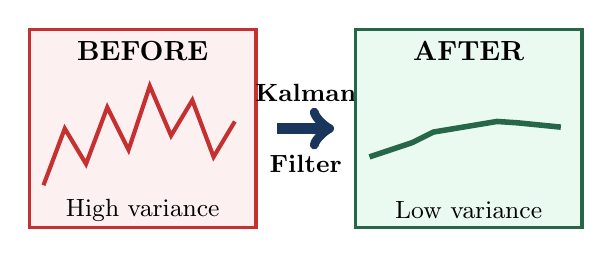
\begin{tikzpicture}[scale=0.9]
    % Before box
    \draw[brickred, very thick, fill=lightred] (0,0) rectangle (3.2,2.8);
    \node[font=\bfseries] at (1.6,2.5) {BEFORE};
    \draw[brickred, thick, line width=1.5pt] (0.2,0.6) -- (0.5,1.4) -- (0.8,0.9) -- (1.1,1.7) -- (1.4,1.1) -- (1.7,2.0) -- (2.0,1.3) -- (2.3,1.8) -- (2.6,1.0) -- (2.9,1.5);
    \node at (1.6,0.25) {\small High variance};
    
    % Arrow
    \draw[->, line width=4pt, navyblue] (3.5,1.4) -- (4.3,1.4);
    \node[font=\bfseries\small] at (3.9,1.9) {Kalman};
    \node[font=\bfseries\small] at (3.9,0.9) {Filter};
    
    % After box
    \draw[forestgreen, very thick, fill=lightgreen] (4.6,0) rectangle (7.8,2.8);
    \node[font=\bfseries] at (6.2,2.5) {AFTER};
    \draw[forestgreen, thick, line width=2pt] (4.8,1.0) -- (5.1,1.1) -- (5.4,1.2) -- (5.7,1.35) -- (6.0,1.4) -- (6.3,1.45) -- (6.6,1.5) -- (6.9,1.48) -- (7.2,1.45) -- (7.5,1.42);
    \node at (6.2,0.25) {\small Low variance};
\end{tikzpicture}
\end{center}

\vspace{0.3em}
\textbf{Features:}
\begin{itemize}[leftmargin=*, nosep, topsep=2pt]
    \item 5 Data Sources: Bitcoin, Temperature, Stocks, Sensor, GPS
    \item Before/After comparison
    \item Adjustable R and Q parameters
    \item Interactive step-by-step calculator
\end{itemize}

\vspace{0.3em}
\colorbox{lightblue}{\parbox{0.95\linewidth}{
\centering\textbf{Try it:} \url{leonathn.github.io/FinalProjectProbability}
}}
}

%==============================================================================
% COLUMN 4: RESULTS & APPLICATIONS
%==============================================================================

\headerbox{\textsf{7. Results \& Validation}}{name=results,column=3,row=0}{
\small
\begin{center}
\begin{tabular}{|l|c|c|}
\hline
\textbf{Metric} & \textbf{Raw} & \textbf{Filtered} \\
\hline
Variance & High & \cellcolor{lightgreen}\textcolor{forestgreen}{\textbf{-40 to -70\%}} \\
\hline
Trend & -- & \cellcolor{lightgreen}\textcolor{forestgreen}{\checkmark Preserved} \\
\hline
Response & -- & \cellcolor{lightgreen}\textcolor{forestgreen}{\checkmark Fast} \\
\hline
Lag & -- & \cellcolor{lightgreen}\textcolor{forestgreen}{Minimal} \\
\hline
\end{tabular}
\end{center}

\vspace{0.3em}
\textbf{Key Findings:}
\begin{enumerate}[leftmargin=*, nosep, topsep=2pt]
    \item Consistent noise reduction across all data types
    \item Filter adapts automatically via Kalman Gain
    \item Underlying trends preserved
    \item Real-time performance achieved
\end{enumerate}
}

\headerbox{\textsf{8. Real-World Applications}}{name=applications,column=3,below=results}{
\small
\begin{itemize}[leftmargin=*, nosep, topsep=2pt]
    \item \textbf{\textcolor{navyblue}{Navigation:}} GPS, autonomous vehicles, drones, spacecraft
    \item \textbf{\textcolor{forestgreen}{Finance:}} Stock prediction, risk assessment, trading
    \item \textbf{\textcolor{goldaccent}{Robotics:}} Sensor fusion, SLAM, motion tracking
    \item \textbf{\textcolor{brickred}{Medical:}} ECG/EEG signal processing
    \item \textbf{Weather:} Temperature, atmospheric modeling
\end{itemize}

\vspace{0.3em}
\colorbox{lightyellow}{\parbox{0.95\linewidth}{
\centering\textit{Apollo 11 used Kalman Filter to reach the Moon!}
}}
}

\headerbox{\textsf{9. Conclusion}}{name=conclusion,column=3,below=applications}{
\small
The Kalman Filter is:

\begin{enumerate}[leftmargin=*, nosep, topsep=2pt]
    \item \textbf{Fundamentally probabilistic} --- Gaussian + Bayes
    \item \textbf{Mathematically elegant} --- only 4 equations
    \item \textbf{Practically powerful} --- proven on real data
    \item \textbf{Widely applicable} --- smartphones to spacecraft
\end{enumerate}

\vspace{0.3em}
\textbf{Future:} Extended Kalman Filter, multi-dimensional states
}

\headerbox{\textsf{References}}{name=references,column=3,below=conclusion}{
\scriptsize
\begin{enumerate}[leftmargin=*, nosep, topsep=2pt]
    \item Kalman, R.E. (1960). \textit{J. Basic Engineering}.
    \item Welch \& Bishop (2006). \textit{UNC Chapel Hill}.
    \item Simon, D. (2006). \textit{Optimal State Estimation}. Wiley.
\end{enumerate}
}

\end{poster}
\end{document}
